%==============================================================================%
%            PRØVE | FORKURS 1P-2P LÆRERUTDANNING | V2016 | UTSATT             %
%==============================================================================%
%
% __/\\\\\\\\\\\\____________________/\\\\\\______________/\\\\\\\\\_____
%  _\/\\\////////\\\_________________\////\\\____________/\\\///////\\\___
%   _\/\\\______\//\\\___________________\/\\\___________\///______\//\\\__
%    _\/\\\_______\/\\\_____/\\\\\\\\_____\/\\\_____________________/\\\/___
%     _\/\\\_______\/\\\___/\\\/////\\\____\/\\\__________________/\\\//_____
%      _\/\\\_______\/\\\__/\\\\\\\\\\\_____\/\\\_______________/\\\//________
%       _\/\\\_______/\\\__\//\\///////______\/\\\_____________/\\\/___________
%        _\/\\\\\\\\\\\\/____\//\\\\\\\\\\__/\\\\\\\\\_________/\\\\\\\\\\\\\\\_
%         _\////////////_______\//////////__\/////////_________\///////////////_
%
%==============================================================================%
%                               MED HJELPEMIDLER                               %
%==============================================================================%

\Del*{m}


%==============================================================================%
%                                 OPPGAVE 2.1                                  %
%==============================================================================%
\Oppgave[2] \points*{2}

Ingrid eier noen aksjer. I dag er verdien av aksjene $\num{80000}$~kroner. Anta
at verdien av aksjene vil øke med $\SI{4.5}{\percent}$ per måned i $6$ av de
$12$ neste månedene. I de andre $6$ månedene vil verdien avta med
$\SI{4.5}{\percent}$ \bigskip

Hva vil aksjene være verdt om ett år?


%==============================================================================%
%                                 OPPGAVE 2.2                                  %
%==============================================================================%
\Oppgave[9]

En tank med melk begynner å lekke. Det er $M(x)$ liter melk i tanken  $x$
minutter etter at lekkasjen starter, der
%
\begin{equation*}
  M(x) = \num{10000} \cdot \num{0.998}^x
  \qquad , \qquad
  0 \leq x \leq 600
\end{equation*}

\begin{oppgaver}
  \Item{2} Gi en praktisk tolkning av tallene $\num{10000}$ og $\num{0.998}$ i
  denne oppgaven.
\end{oppgaver}

\begin{oppgaver}
  \Item{2} Bruk graftegner til å tegne grafen til $M$.
\end{oppgaver}

En funksjon $S$ er gitt ved
%
\begin{equation*}
  S(x) = \num{10000} \cdot (1 - \num{0.998}^x)
  \qquad , \qquad
  0 \leq x \leq 600
\end{equation*}

\begin{oppgaver}
  \Item{2} Tegn grafen til $S$ i samme koordinatsystem som grafen til $M$.
  Bestem skjæringspunktet mellom de to grafene.
\end{oppgaver}

\begin{oppgaver}
  \Item{1} Bestem $S(480)$. Forklar hvilken informasjon  $S(x)$ gir oss.
\end{oppgaver}

\begin{oppgaver}
  \Item{2} Bestem den momentane vekstfarten til funksjonen $M$ når $x=180$.
  Bestem den momentane vekstfarten til funksjonen $S$ når $x=180$. Gi en
  praktisk tolkning av disse svarene.
\end{oppgaver}


%==============================================================================%
%                                 OPPGAVE 2.3                                  %
%==============================================================================%
\Oppgave[5]

\begin{figure}[H]
  \centering
  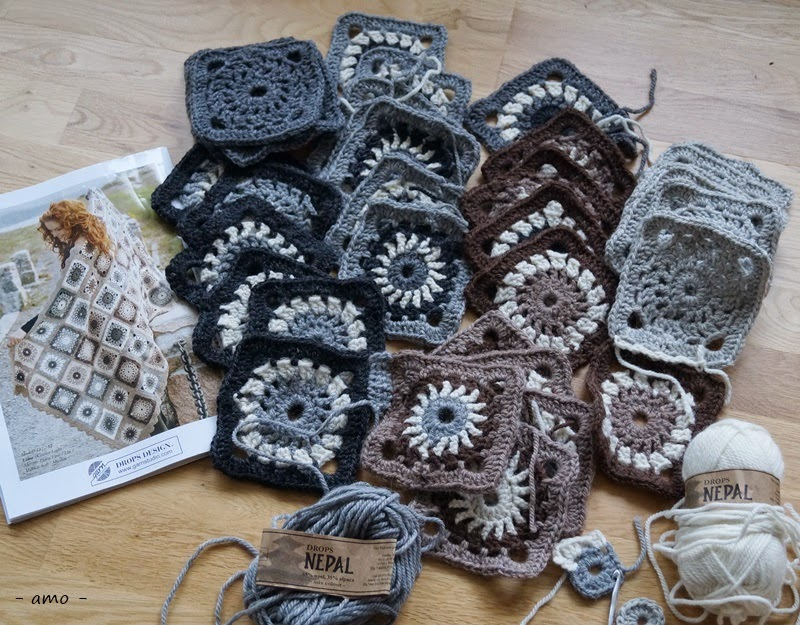
\includegraphics[width=0.6\textwidth]{Forkurs-1p-2p-laererutdanning-2016-V-U-oppgave-2-3-lappeteppe.jpg}
\end{figure}

Sara hekler lapper til et lappeteppe. nedenfor viser hvor mange ferdige lapper
hun hadde $1$, $6$, $15$ og $20$ dager etter hun startet å hekle.

\begin{table}[H]
  \centering
  \label{tab:Forkurs-1p-2p-laererutdanning-2016-V-U-oppgave-2-3}
  \begin{tabular}{|l| *{4}{S[table-format=2.0]|}} \hline
    \Cellcolor Antall dager etter start & 1 &  6 & 15 & 20 \\ \hline
    \Cellcolor Antall ferdige lapper    & 5 & 16 & 28 & 35 \\ \hline
  \end{tabular}
\end{table}

\begin{oppgaver}
  \Item{2} Bruk regresjon til å bestemme en potensfunksjon som viser hvor mange
  ferdige lapper hun hadde $x$~dager etter at hun startet å hekle.
  \label{opg:Forkurs-1p-2p-laererutdanning-2016-V-U-oppgave-2-3a}
\end{oppgaver}

\begin{oppgaver}
  \Item{1} Hvor mange dager vil det gå før sara har $100$ ferdige lapper ifølge
  funksjonen i \cref{opg:Forkurs-1p-2p-laererutdanning-2016-V-U-oppgave-2-3a}?
\end{oppgaver}

\begin{oppgaver}
  \Item{2} Bestem gjennomsnittlig vekstfart fra $x=14$ til $x=50$. Gi en
  praktisk tolkning av dette svaret.
\end{oppgaver}


%==============================================================================%
%                                 OPPGAVE 2.4                                  %
%==============================================================================%
\Oppgave[3]

I en klasse ved en idrettslinje er det $24$ elever. $16$ av elevene spiller
fotball. $10$ av elevene spiller håndball. $2$ av elevene spiller verken
fotball eller håndball. Tenk deg at du skal trekke én elev fra klassen
tilfeldig.

\begin{oppgaver}
  \Item{2} Bestem sannsynligheten for at du kommer til å trekke en elev som
  spiller håndball, men ikke fotball.
\end{oppgaver}

Tenk deg at du har trukket en elev som spiller fotball.

\begin{oppgaver}
  \Item{1} Bestem sannsynligheten for at eleven også spiller håndball.
\end{oppgaver}


%==============================================================================%
%                                 OPPGAVE 2.5                                  %
%==============================================================================%
\Oppgave[3]

En gryte har form som en sylinder med diameter $\SI{21}{\centi\metre}$ og høyde
$\SI{29}{\cm}$.

\begin{oppgaver}
  \Item{1} Hvor mange liter rommer gryta?
\end{oppgaver}

Tenk deg at $\cfrac{3}{4}$ av gryta er fylt med gelé. Geneen skal fylles i
kjegleformede glass. Kjeglene har diameter $\SI{10}{\cm}$ og høyde
$\SI{12}{\centi\metre}$.

\begin{oppgaver}
  \Item{2} Hvor mange glass trenger vi?
\end{oppgaver}


%==============================================================================%
%                                 OPPGAVE 2.6                                  %
%==============================================================================%
\Oppgave[3]

\begin{table}[H]
  \centering
  \caption{}
  \label{tab:Forkurs-1p-2p-laererutdanning-2016-V-U-oppgave-2-6}
  \begin{tabular}{| l | S[table-format=4.0] | S[table-format=4.0] |}
    \hline
    \Rowcolor \headerstrut & 2014 & 2015 \\ \hline
    \Rowcolor Måned \headerstrut & {Forbruk $\si{\kilo\watt\hour}$} & {Forbruk
    $\si{\kilo\watt\hour}$}   \\ \hline
     \Cellcolor Januar  & 1936 & 1704  \\ \hline
     \Cellcolor Februar & 846 & 1505   \\ \hline
     \Cellcolor Mars    & 2144 & 1610  \\ \hline
     \Cellcolor April   & 1581 & 1422  \\ \hline
     \Cellcolor Mai     & 1499 & 1499  \\ \hline
     \Cellcolor Juni    & 521 & 1083   \\ \hline
  \end{tabular}
\end{table}

Tabellen ovenfor viser hvor mye elektrisk energi en familie brukte hver måned
i første halvdel av $2014$ og i første halvdel av $2015$.

\begin{oppgaver}
    \Item{2} Bestem gjennomsnittet og standardavviket for forbruket per måned i
    første halvdel av $2014$ og i første halvdel av $2015$.
\end{oppgaver}

\begin{oppgaver}
    \Item{1} Hva forteller standardavvikene om forbruket i første halvdel
    av$2014$ sammenliknet med forbruket i første halvdel av $2015$?
\end{oppgaver}

\clearpage
%==============================================================================%
%                                 OPPGAVE 2.7                                  %
%==============================================================================%
\Oppgave[4]

Import AS kjøper varer fra et utenlandsk firma og selger varene videre til
butikker i Norge. For å bestemme utsalgsprisen til butikkene gjør Import AS
følgende beregninger:

\begin{center}
  \begin{tabular}{@{}c c @{}c l @{}c}
    &   &  & Innkjøpspris & \\
    & + &  & Kostnader til pransport, toll og merverdiavgift & \\
    & + &  & Fortjeneste & \\ \midrule
    & = &  & Utsalgspris & \\
  \end{tabular}
\end{center}


Innkjøpsprisen er den prisen (i norske kroner) som Import AS betaler til det
utenlandske firmaet for en vare. \bigskip

Import AS regner med at de totale kostnadene til transport, toll og
merverdiavgift for en vare tilsvarer $\SI{60}{\percent}$ av varens innkjøpspris.
\bigskip

For varer som har innkjøpspris lavere enn $\num{1000}$~kroner, beregner Import
AS en fortjeneste på $\SI{30}{\percent}$ av innkjøpsprisen. For alle andre varer
beregnes en fortjeneste på $\SI{25}{\percent}$ av innkjøpsprisen.

\begin{oppgaver}
    \Item{3} Lag ett regneark som Import AS kan bruke til å beregne
      utsalgsprisen for en vare.  Når firmaet legger inn innkjøpsprisen, skal
      regnearket beregne kostnader, fortjeneste og utsalgspris på grunnlag av
      innkjøpsprisen som legges inn.
    \label{opg:Forkurs-2016-H-oppgave-2.7a}
\end{oppgaver}

\begin{oppgaver}
  \Item{1} Bruk regnearket du laget i \cref{opg:Forkurs-2016-H-oppgave-2.7a},
    til å beregne utsalgsprisen til en vare med innkjøpspris $800$ kroner og
    utsalgsprisen til en vare med innkjøpspris $\num{1200}$~kroner.
\end{oppgaver}

%==============================================================================%
%                                 OPPGAVE 2.8                                  %
%==============================================================================%
\Oppgave[7]
\vspace*{-1cm}
\begin{figure}[H]
   \centering
   \foreach \X in {1,...,4}
   {\begin{subfigure}[b]{\X.5cm}
       \centering
       \staircase{\X}
       \caption*{$F_\X$}
   \end{subfigure}}
   \caption{}
   \label{fig:Forkurs-1p-2p-laererutdanning-2016-V-U-oppgave-2-8a}
\end{figure}

I \cref{fig:Forkurs-1p-2p-laererutdanning-2016-V-U-oppgave-2-8a} ser du fire
figurer $F_1$, $F_2$, $F_3$ og $F_4$. Figurene er satt sammen av små svarte,
røde og blå pinner. Tenk deg at du skal fortsette å lage figurer etter samme
mønster.

\begin{oppgaver}
  \Item{1} Hvor mange svarte pinner vil det være i $F_5$?
\end{oppgaver}

\begin{oppgaver}
  \Item{2} Bestem et uttrykk for antall svarte pinner i figur $F_n$ uttrykt
  ved $n$.
\end{oppgaver}

Elise arbeider med å bestemme summen av røde og blå pinner i figur $F_n$. Hun
har lage skissene vist nedenfor i
\cref{fig:Forkurs-1p-2p-laererutdanning-2016-V-U-oppgave-2-8b}.

\begin{figure}[!h]
  \centering
  \foreach \X in {1,...,4}
  {\begin{subfigure}[b]{\X.5cm}
      \centering
      \staircaseSum{\X}
      \caption*{$F_\X$}
  \end{subfigure}}
  \caption{}
  \label{fig:Forkurs-1p-2p-laererutdanning-2016-V-U-oppgave-2-8b}
\end{figure}

\begin{oppgaver}
  \Item{2} Bestem et uttrykk for summen av antall røde og antall blå pinner i
  figur $F_n$ uttrykt ved $n$.
\end{oppgaver}

Tenk deg at du har $\num{600}$~svarte, $\num{1000}$~røde og $\num{1200}$ blå
pinner. Du skal lage en figur etter samme mønster som ovenfor. Figuren skal være
så stor som mulig.

\begin{oppgaver}
  \Item{2} Hvor mange pinner vil denne figuren inneholde totalt?
\end{oppgaver}
